\begin{frame}[t]{\id{e95e3d8e}\enspace Arm B reconstructed an eight-by-eight tile}
\med
The solver tried tile heights and widths in order, up to 100 cells per tile. It accepted the first shape for which all visible colors agreed at positions with the same row and column remainders.
\par\vspace{1mm}
\begin{center}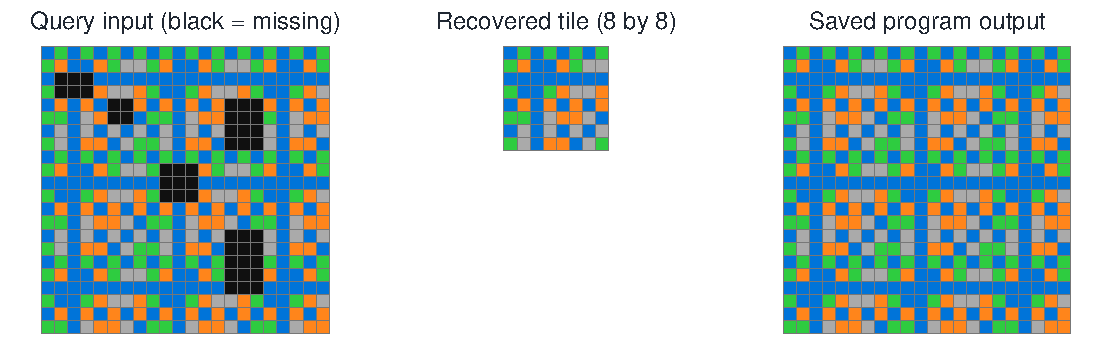
\includegraphics[height=46mm]{python-case-audit/solved-tile.pdf}\end{center}
\med
\texttt{out[r][c] = tile[r \% ph][c \% pw]}\par\vspace{1.5mm}
The first candidate matched all three demonstrations. On the query it filled all 46 holes and matched all 484 cells. B used 908 tokens, about 10:02 of active time and zero exploratory Python calls.
\vfill
\smallbody The direct-answer runs also solved this task with checkpoint-660 and both BF16 sampling settings. NF4 base wrote the right cells and omitted the outer JSON list.
\end{frame}

\begin{frame}[t]{\id{e95e3d8e}\enspace Arm A identified repetition and kept describing it}
\med
The same input reached both arms. A recognized the missing patches and the first demonstration's five-by-five period. Its saved text continued through the second demonstration.
\par\vspace{4mm}
\begin{tabular}{@{}p{94mm}rr@{}}
\toprule
Recorded first pass & Arm A & Arm B\\
\midrule
Generated tokens & 1,123 & 908\\
Charged generation time & 12:03 & 10:02\\
Completed solver candidates & 0 & 1\\
Demonstrations matched & Unexecuted & 3 / 3\\
Held-out query & No grid & 484 / 484 cells\\
\bottomrule
\end{tabular}
\par\vspace{4mm}
\med The controller ended A's reasoning phase at 512 tokens. Its next 610 tokens contained prose and grid values. When the generation allowance expired, there was no \texttt{solve(grid)} function to execute during the three-minute reserve.
\vfill
\smallbody The saved prefix establishes where A stopped. Its eventual answer with more time is unknown.
\end{frame}
